%!TEX root = ../main.tex
%%%%%%%%%%%%%%%%%%%%%%%%%%%%%%%%%%%%%%%%
%
%LEZIONE 27/04/2016 - NONA SETTIMANA (2)
%
%%%%%%%%%%%%%%%%%%%%%%%%%%%%%%%%%%%%%%%%
\chapter{Superfici e integrali di superficie}
%%%%%%%%%%%%%%%%%%%%%%%%%%
%CONTROESEMPIO DI SCHWARZ%
%%%%%%%%%%%%%%%%%%%%%%%%%%
\section{Controesempio di Schwarz}

Nei paragrafi precedenti abbiamo osservato come la lunghezza di una curva \(\g\) possa essere definita come l'estremo superiore della lunghezza delle spezzate, oppure, nel caso la curva sia \(C^1\), come
\[
	\int\limits_\g \norma{\dot{\g}(t)}\,\dd t.
\]
In questo paragrafo ci occuperemo di studiare le aree delle superfici.
Volendo fare un'analogia con le curve, ci aspettiamo che l'area di una superficie possa essere studiata sia come limite della aree di triangolazioni sempre più fini, che tramite una parametrizzazione ed una formula.

Nella prossima proposizione vedremo come la prima intuizione risulti sbagliata.

\begin{prop}{Controesempio di Schwarz}{controesempioSchwarz}\index{Controesempio di Schwarz}
	Consideriamo \(S\) il cilindro di raggio \(r\) e altezza \(h\).
	Supponiamo di triangolarne la superficie, allora l'area della superficie dipende dalla triangolazione.
\end{prop}

\begin{proof}
	Supponiamo di dividere \(S\) in \(m\) semicilindri di altezza \(\frac{h}{m}\) ciascuno.

	Per ogni semicilindro, dividiamo le circonferenze di base in \(n\) archi di lunghezza congruente in modo tale che gli estremi di ogni arco costituiscano i vertici del triangolo iscritto nella superficie laterale del semicilindro, come nella figura \ref{fig:controesempioSchwarz}.

	Chiaramente gli archi di due circonferenze successive saranno sfasati di un mezzo arco.

	Supponiamo che \(\triangle BAC\) sia uno qualsiasi dei triangoli iscritti in un semicilindro.
	Definiamo \(D\) e \(E\) rispettivamente come i punti medi del segmento \(\overline{BC}\) e dell'arco \(\overset{\frown}{BC}\).

	Sia \(O\) il centro della circonferenza che contiene l'arco \(\overset{\frown}{BC}\), così che \(\triangle BOC\) sia parallelo alla base del cilindro.
	Per costruzione avremo
	\[
		\q = B\hat{O}D = \frac{\p}{n} \qquad\text{e}\qquad \abs{\overline{BC}} = 2r \sin \q = 2r \sin \frac{\p}{n}.
	\]
	Per trovare l'area di \(\triangle BAC\) è necessario, per prima cosa, applicare il teorema di Pitagora a \(\triangle ADE\) per calcolare l'altezza \(\abs{\overline{AD}}\):
	\[
		\abs{\overline{DE}} = \abs{\overline{OE}} - \abs{\overline{OD}} = r-r \cos \q = r \left( 1-\cos \frac{\p}{n} \right),
	\]
	da cui
	\[
		\abs{\overline{AD}}^2 = \abs{\overline{AE}}^2 + \abs{\overline{DE}}^2 = \left( \frac{h}{m} \right)^2 + r^2 \left( 1-\cos \frac{\p}{n} \right)^2,
	\]
	quindi
	\[
		\begin{split}
			\text{area}(\triangle BAC) & = \frac{1}{2} \abs{\overline{BC}} \abs{\overline{AD}} = \frac{1}{2} \left( 2r \sin \frac{\p}{n} \right) \sqrt{\left( \frac{h}{m} \right)^2 + r^2 \left( 1- \cos \frac{\p}{n} \right)^2}\\
			& = r\sin \frac{\p}{n} \sqrt{\left( \frac{h}{m} \right)^2 + r^2 \left( 1- \cos \frac{\p}{n} \right)^2}.
		\end{split}
	\]
	In ognuno degli \(m\) semicilindri ci sono \(2n\) di questi triangoli, i quali sono tutti congruenti tra loro.
	In particolare la nostra triangolazione ha prodotto \(2\,m\,n\) di tali triangoli.
	Quindi l'area di \(S\) in funzione di \(m\) e \(n\) sarà:
	\[
		A(m,n) = 2m\,n \left(r\sin \frac{\p}{n}\right) \sqrt{\left( \frac{h}{m} \right)^2 + r^2 \left( 1- \cos \frac{\p}{n} \right)^2}.
	\]
	Se poniamo \(m=q\,n^2\) otteniamo
	\[
		\abs{A(m,n)} = \abs*{2q\,n^3 \left( r \sin \frac{\p}{n} \right) \sqrt{\frac{h^2}{q^2 n^4} + r^2 \left( 1-\cos \frac{\p}{n} \right)^2}}.
	\]
	Ora per \(n \to +\infty\) avremo
	\[
		\sin \frac{\p}{n} \cong \frac{\p}{n} \qquad\text{e}\qquad 1-\cos \frac{\p}{n} \cong \frac{1}{2} \frac{\p^2}{n^2},
	\]
	per cui
	\[
		\abs{A(m,n)} \cong \abs*{2q\,r\,\p \sqrt{ \frac{r^2 \p^4}{4}+ \frac{h^2}{q^2}}}.
	\]
	Quindi l'area del cilindro dipende da \(q\), per cui dipende dalla triangolazione.
	Ne segue che questo metodo non è valido.
\end{proof}

\begin{figure}[tp]
	\begin{centering}
		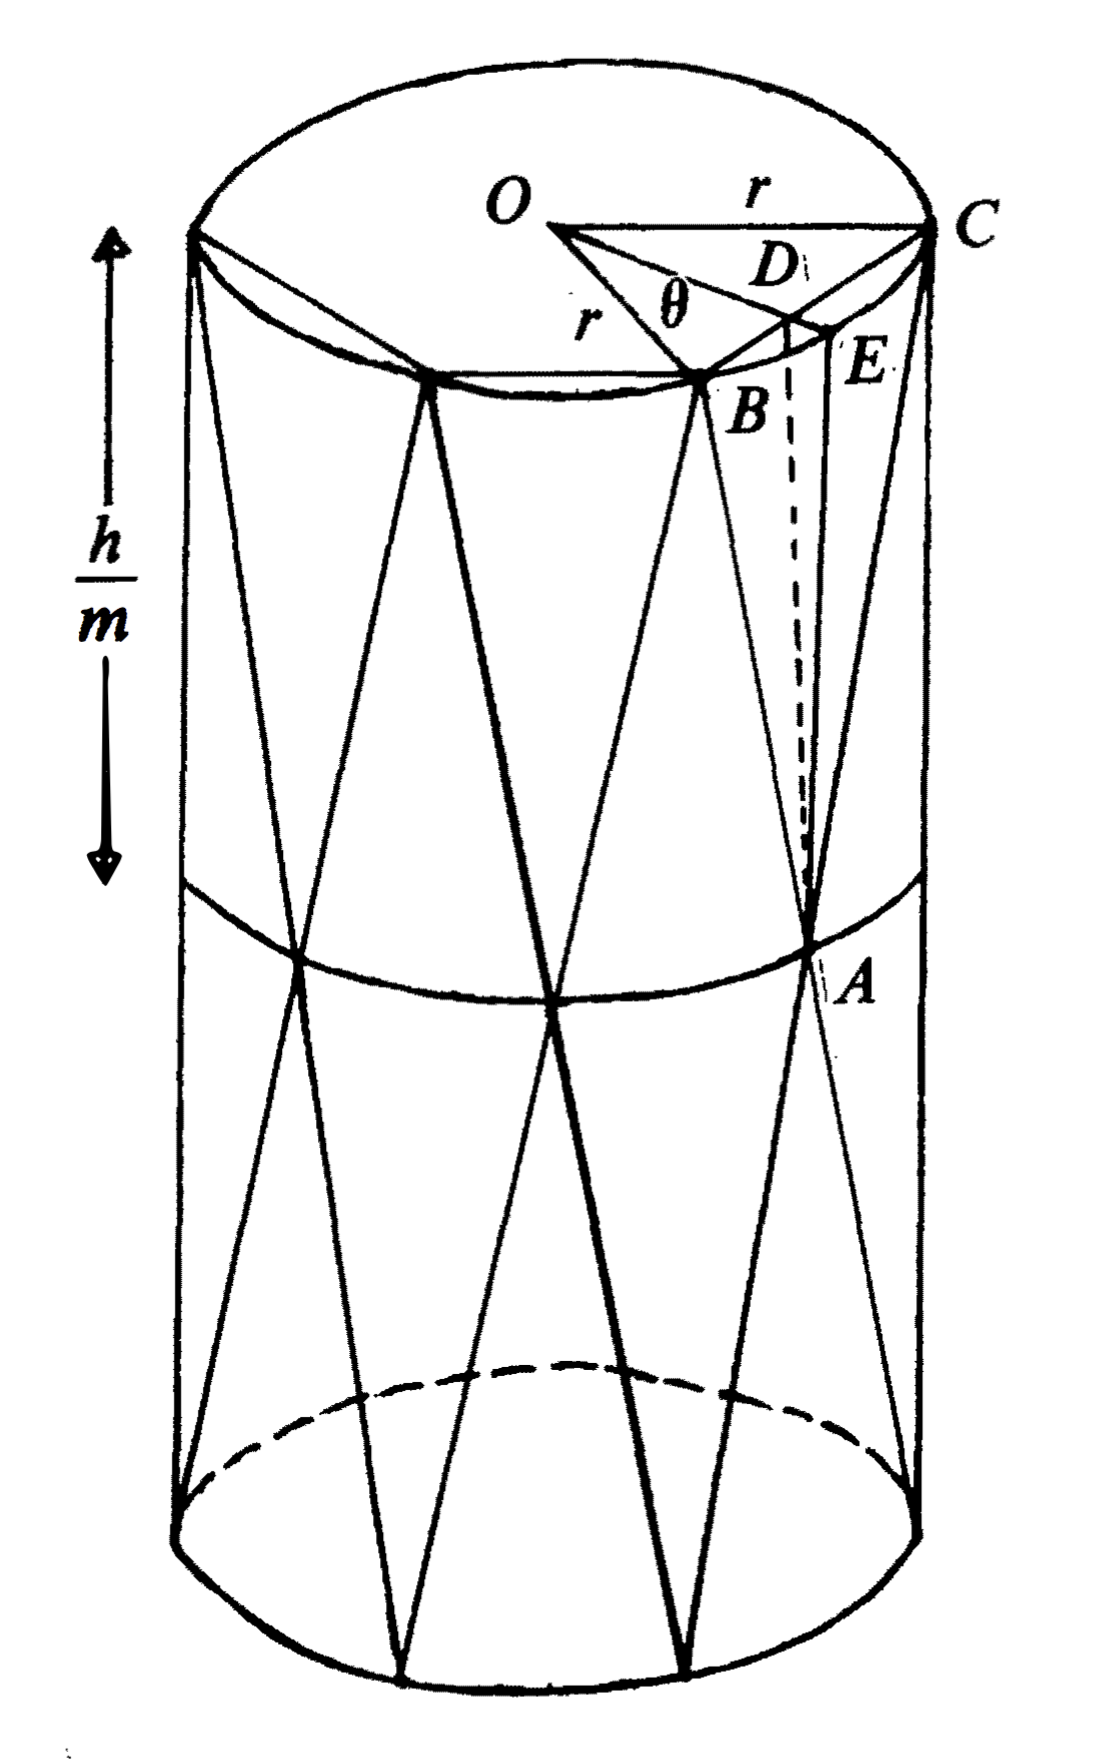
\includegraphics[height = 75mm]{controesempioSchwarz.png}
		\caption{La triangolazione di un cilindro di raggio \(r\) e altezza \(h\).}
		\label{fig:controesempioSchwarz}
	\end{centering}
\end{figure}
%%%%%%%%%%%%%%%%%%%%%%%%%%%%%%%%%%%%%%%%%%
%
%LEZIONE 03/05/2016 - DECIMA SETTIMANA (2)
%
%%%%%%%%%%%%%%%%%%%%%%%%%%%%%%%%%%%%%%%%%%
%%%%%%%%%%%%%%%%%%%%%%%%%
%INTEGRALI DI SUPERFICIE%
%%%%%%%%%%%%%%%%%%%%%%%%%
\section{Integrali di superficie}

\begin{defn}{Superficie regolare}{superficieRegolare}\index{Superficie regolare}
	Sia \(\Omega\subseteq\R^2\) un aperto connesso.
	Una \emph{superficie regolare}, parametrizzata, di \(\R^3\) è una mappa \(\j\in C^1(\Omega,\R^3)\) che sia iniettiva e tale che
	\[
		\frac{\pd \j(u,v)}{\pd u} \wedge \frac{\pd \j(u,v)}{\pd v} \neq 0,\,\fa (u,v)\in \Omega.
	\]
\end{defn}

\begin{notz}
	In questo caso la notazione del prodotto \(\wedge\) rappresenta il ben noto prodotto vettoriale.
\end{notz}

\begin{oss}
	In altre parole, la condizione sulle derivate parziali può essere riassunta nella lineare indipendenza di
	\[
		\begin{pmatrix}
			\frac{\pd \j_1(u,v)}{\pd u} \\
			\frac{\pd \j_2(u,v)}{\pd u} \\
			\frac{\pd \j_3(u,v)}{\pd u}
		\end{pmatrix}
		\qquad\text{e}\qquad
		\begin{pmatrix}
			\frac{\pd \j_1(u,v)}{\pd v} \\
			\frac{\pd \j_2(u,v)}{\pd v} \\
			\frac{\pd \j_3(u,v)}{\pd v}
		\end{pmatrix}
	\]
\end{oss}

\begin{defn}{Integrale di una funzione lungo una superficie}{integraleDiSuperficie}\index{Integrale!di superficie}
	Siano \(\Omega\subseteq\R^2\) un aperto e \(\j\) una superficie regolare su \(\Omega\).
	Sia \(f\colon \j(\Omega) \to \R\) una funzione continua.
	L'integrale di \(f\) lungo \(\j(\Omega)\) si definisce come
	\[
		\int\limits_{\j(\Omega)} f\,\dd s = \int\limits_\Omega f\big(\j(u,v)\big) \norma*{\frac{\pd \j(u,v)}{\pd u}\wedge \frac{\pd \j(u,v)}{\pd v}}\,\dd u\,\dd v.
	\]
\end{defn}

\begin{ese}
	Calcoliamo la superficie della sfera di raggio \(R\).
	Utilizziamo la parametrizzazione canonica che ci viene suggerita dalle coordinate sferiche
	\[
		\j\colon (0,\p) \times S^1 \to \R^3, \begin{pmatrix}\y\\\q\end{pmatrix} \mapsto \begin{pmatrix}
			R \sin \y \cos \q \\
			R \sin \y \sin \q \\
			R \cos \y
		\end{pmatrix}
	\]
	Calcoliamo quindi il prodotto vettore delle derivate parziali
	\[
		\begin{split}
			\frac{\pd \j(\y,\q)}{\pd \y} \wedge \frac{\pd \j(\y,\q)}{\pd \q} & = \det 	\begin{pmatrix}
				\bar{i}            & \bar{j}           & \bar{k}    \\
				R \cos \y \cos \q  & R \cos \y \sin \q & -R \sin \y \\
				-R \sin \y \sin \q & R \sin \y \cos \q & 0
			\end{pmatrix}\\
			& = \bar{i} (R^2 \sin^2 \y \cos \q) + \bar{j}(R^2 \sin^2\y \sin \q) + \bar{k}(R^2\sin \y \cos \y)\\
			& = R \sin \y (R \sin \y \cos \q\, \bar{i} + R\sin \y \sin \q\, \bar{j} + R\cos \y\,\bar{k})\\
			& = R \sin \y \j(R)\graffito{con \(\j(R)\) denotiamo in maniera compatta il vettore sulla sfera di raggio \(R\)}.
		\end{split}
	\]
	Per cui la superficie della sfera è
	\[
		\begin{split}
			\int\limits_{\j(\Omega)}\dd s & = \int\limits_\Omega \norma*{\frac{\pd \j}{\pd \y}\wedge \frac{\pd \j}{\pd \q}}\,\dd \y\,\dd \q\\
			& = \int\limits_\Omega R^2\sin \y\,\dd \y\,\dd \q = R^2 \int_0^\p \sin \y\,\dd \y \int_0^{2\p} \dd \q\graffito{utilizzando le formule di riduzione}\\
			& = 4\p\,R^2.
		\end{split}
	\]
\end{ese}

\begin{prop}{Il prodotto vettore è ortogonale alla superficie}{prodottoVettoreOrtogonaleSuperficie}
	Sia \(\j \colon \Omega \to \R^3\) una superficie regolare.
	Allora
	\[
		\frac{\pd \j}{\pd u} \wedge \frac{\pd \j}{\pd v},
	\]
	è ortogonale alla superficie.
\end{prop}

\begin{proof}
	Possiamo riformulare la tesi dicendo che se \(\g\colon [-1,1] \to \j(\Omega)\) è una curva di classe \(C^1\) sulla superficie, si deve avere
	\[
		\dot{\g}(t) \perp \left( \left.\frac{\pd \j}{\pd u}\right|_{\g(t)} \wedge \left.\frac{\pd \j}{\pd v}\right|_{\g(t)} \right).
	\]
	Infatti \(\dot{\g}(t)\) rappresenta il vettore tangente alla superficie in \(\g(t)\).

	Ora se \(\j\colon \Omega \to \R^3\) posso scrivere \(\g = \j \circ \tilde{\g}\) dove \(\tilde{\g}\colon [-1,1] \to \Omega\).
	In altre parole, prendo una curva su \(\Omega\) e la mappo tramite \(\j\) sulla superficie \(\j(\Omega)\).

	Supponiamo di avere le seguenti parametrizzazioni
	\[
		\j(u,v) = 	\begin{pmatrix}
			x(u,v) \\
			y(u,v) \\
			z(u,v)
		\end{pmatrix}
		\qquad\text{e}\qquad
		\tilde{\g}(t) = \begin{pmatrix}
			u(t) \\
			v(t)
		\end{pmatrix}
	\]
	Applicando la regola della catena avremo
	\[
		\begin{split}
			\dot{\g}(t) & = \frac{\dd}{\dd t} \j \circ \tilde{\g}(t) =  \left.	\begin{pmatrix}
				\frac{\pd x}{\pd u} & \frac{\pd x}{\pd v} \\
				\frac{\pd y}{\pd u} & \frac{\pd y}{\pd v} \\
				\frac{\pd z}{\pd u} & \frac{\pd z}{\pd v}
			\end{pmatrix}\right|_{\tilde{\g}(t)}
			\begin{pmatrix}
				\dot{u}(t) \\
				\dot{v}(t)
			\end{pmatrix}\\
			& = \dot{u}(t)  \begin{pmatrix}
				\frac{\pd x}{\pd u}\big(\g(t)\big) \\
				\frac{\pd y}{\pd u}\big(\g(t)\big) \\
				\frac{\pd z}{\pd u}\big(\g(t)\big)
			\end{pmatrix}
			+ \dot{v}(t)	\begin{pmatrix}
				\frac{\pd x}{\pd v}\big(\g(t)\big) \\
				\frac{\pd y}{\pd v}\big(\g(t)\big) \\
				\frac{\pd z}{\pd v}\big(\g(t)\big)
			\end{pmatrix}
		\end{split}
	\]
	Ora, entrambi i vettori delle derivate parziali sono perpendicolari al prodotto vettore calcolato in \(\g(t)\)\graffito{per la definizione di prodotto vettore}, per cui
	\[
		\dot{\g}(t) \perp \left( \left.\frac{\pd \j}{\pd u}\right|_{\g(t)} \wedge \left.\frac{\pd \j}{\pd v}\right|_{\g(t)} \right),
	\]
	in quanto combinazione lineare di vettori perpendicolari.
\end{proof}

\begin{ese}
	Calcoliamo la superficie del toro bidimensionale.
	Supponiamo che \(R>0\) sia la distanza del centro del tubo al centro del toro e che \(r>0\) sia il raggio del tubo.
	Una possibile parametrizzazione è la seguente
	\[
		\j \colon S^1 \times S^1 \to \R^3, \begin{pmatrix}t\\\q\end{pmatrix} \mapsto 	\begin{pmatrix}
			(R+r\cos t)\cos \q \\
			(R+r\cos t)\sin \q \\
			r\sin t
		\end{pmatrix}
	\]
	Troviamo il prodotto vettore
	\[
		\begin{split}
			\frac{\pd \j(t,\q)}{\pd t} \wedge \frac{\pd \j(t,\q)}{\pd \q} & = \det  \begin{pmatrix}
				\bar{i}             & \bar{j}            & \bar{k}  \\
				-r \sin t \cos \q   & -r \sin t \sin \q  & r \cos t \\
				-(R+r\cos t)\sin \q & (R+r\cos t)\cos \q & 0
			\end{pmatrix}\\
			& = -\bar{i}\big(r(R+r\cos t)\cos t\cos \q\big) -\bar{j}\big(r(R+r\cos t)\cos t\sin \q\big) \\
			& -\bar{k}\big(r(R+r\cos t)\sin t\big)\\
			& = r(R+r\cos t)[-\cos t \cos \q\, \bar{i} - \cos t \sin \q\, \bar{j} - \sin t\, \bar{k}].
		\end{split}
	\]
	Per cui la superficie del toro è
	\[
		\begin{split}
			\int\limits_{\j(\Omega)}\dd s & = \int\limits_\Omega \norma*{\frac{\pd \j}{\pd t} \wedge \frac{\pd \j}{\pd \q}}\,\dd t\,\dd \q\\
			& = \int\limits_\Omega (R+r\cos t)r\,\dd t\,\dd \q = r \int_0^{2\p} \dd \q \int_0^{2\p} (R+r\cos t)\,\dd t\graffito{per le formule di riduzione}\\
			& = 4\p^2 R\, r.
		\end{split}
	\]
\end{ese}

\begin{ese}
	Calcoliamo la superficie del cono di altezza \(\l\).
	Sfruttiamo la parametrizzazione suggerita dalle coordinate cilindriche
	\[
		\j\colon (0,1) \times S^1 \to \R^3, \begin{pmatrix}\r\\\q\end{pmatrix} \mapsto  \begin{pmatrix}
			\r \cos \q \\
			\r \sin \q \\
			\l\,\r
		\end{pmatrix}
	\]
	Troviamo il prodotto vettore
	\[
		\begin{split}
			\frac{\pd \j}{\pd \r} \wedge \frac{\pd \j}{\pd \q} & = \det \begin{pmatrix}
				\bar{i}     & \bar{j}    & \bar{k} \\
				\cos \q     & \sin \q    & \l      \\
				-\r \sin \q & \r \cos \q & 0
			\end{pmatrix}\\
			& = -\bar{i}(\l\,\r \cos \q) - \bar{j}(\l\,\r \sin \q) + \bar{k} (\r).
		\end{split}
	\]
	Quindi la superficie del cilindro è
	\[
		\begin{split}
			\int\limits_{\j(\Omega)}\dd s & = \int\limits_\Omega \norma*{\frac{\pd \j}{\pd \r} \wedge \frac{\pd \j}{\pd \q}}\,\dd \r\,\dd \q\\
			& = \int\limits_\Omega \r\sqrt{\l^2+1}\,\dd \r\,\dd \q = \sqrt{\l^2+1} \int_0^{2\p}\dd \q \int_0^1 \r\,\dd \r\\
			& = \p\sqrt{\l^2+1}.
		\end{split}
	\]
\end{ese}
%%%%%%%%%%%%%%%%%%%%%%%%%%%%%%%%%%%%%%%%%%
%
%LEZIONE 03/05/2016 - DECIMA SETTIMANA (2)
%
%%%%%%%%%%%%%%%%%%%%%%%%%%%%%%%%%%%%%%%%%%
\begin{ese}[Finestra di Viviani]
	Consideriamo la seguente superficie determinata dall'intersezione di una sfera con un cilindro nel semispazio superiore,
	\[
		F = \Set{(x,y,z) | x^2+y^2+z^2 = r^2, \left( x- \frac{r}{2} \right)^2 + y^2 \le \frac{r^2}{4},z>0}.
	\]
	Per il calcolo dell'area della superficie sfrutteremo le coordinate cilindriche
	\[
		\j\colon (0,+\infty) \times S^1 \times \R \to \R^3\setminus\Set{(0,0,z) | z\in \R}, \begin{pmatrix}\r\\\q\\\l\end{pmatrix} \mapsto \begin{pmatrix}
			\r\cos\q \\
			\r\sin\q \\
			\l
		\end{pmatrix}
	\]
	Per la parametrizzazione consideriamo la proiezione sul piano \(x y\), otteniamo le condizioni
	\[
		0 \le \r \le r\cos \q \qquad\text{e}\qquad -\frac{\p}{2} < \q < \frac{\p}{2}.
	\]
	Quindi una parametrizzazione della finestra di Viviani è la seguente
	\[
		\y\colon \Set{(\r,\q) | -\frac{\p}{2}<\q<\frac{\p}{2}, 0<\r<r\cos\q} \to \R^3, \begin{pmatrix}\r\\\q\end{pmatrix} \to 	\begin{pmatrix}
			\r \cos \q \\
			\r \sin \q \\
			\sqrt{r^2-\r^2}
		\end{pmatrix}
	\]
	Per il calcolo dell'area è quindi sufficiente trovare il prodotto vettore e calcolare l'integrale di superficie.
\end{ese}
%%%%%%%%%%%%%%%%%%%%%%%%%%%%%%%%%%
%SIGNIFICATO DEL PRODOTTO VETTORE%
%%%%%%%%%%%%%%%%%%%%%%%%%%%%%%%%%%
\section{Significato del prodotto vettore}

Per come abbiamo definito l'integrale lungo una superficie, è lecito domandarsi perché
\[
	\dd S = \norma*{\frac{\pd \y}{\pd u} \wedge \frac{\pd \y}{\pd v}}
\]
In questo paragrafo forniremo una spiegazione inizialmente empirica su \(\R^2\), per poi estenderci al caso generale tramite un teorema di indipendenza rispetto alla parametrizzazione.

Supponiamo di avere due aperti \(\Omega,\Omega'\subseteq\R^2\) e una mappa \(\y\) che manda \(\Omega'\) in \(\Omega\).
Tali aperti possono anche essere pensati come due superfici "piatte" in \(\R^3\), ad esempio parametrizzandole come
\[
	\begin{pmatrix}u\\v\end{pmatrix} \mapsto 	\begin{pmatrix}
		x(u,v) \\
		y(u,v) \\
		0
	\end{pmatrix}
\]
Mostriamo ora che la formula dell'area delle superfici ci fornisce l'area di \(\Omega\).
Calcoliamo il prodotto vettore
\[
	\begin{split}
		\frac{\pd \y}{\pd u} \wedge \frac{\pd \y}{\pd v} & = \det 	\begin{pmatrix}
			\bar{i} & \bar{j} & \bar{k} \\
			\pd_u x & \pd_u y & 0       \\
			\pd_v x & \pd_v y & 0
		\end{pmatrix}\\
		& = 0\bar{i} + 0\bar{j} + \bar{k}(\pd_u x \pd_v y - \pd_u y \pd_v x)\\
		& = \bar{k} \det \frac{\pd(x,y)}{\pd(u,v)}.
	\end{split}
\]
Ovvero
\[
	\norma*{\frac{\pd \y}{\pd u} \wedge \frac{\pd \y}{\pd v}} = \abs*{\frac{\pd(x,y)}{\pd(u,v)}},
\]
che, tramite la formula dell'integrale lungo una superficie, ci fornisce
\[
	\abs{\Omega} = \int\limits_{\Omega'} \abs*{\frac{\pd(x,y)}{\pd(u,v)}}\,\dd u\,\dd v.
\]
Quindi in \(\R^2\) tale formula è una restrizione della definizione di area di una superficie tramite cambiamento di variabile.

La ragione per cui questo vale anche in \(\R^3\) viene dal teorema seguente

\begin{teor}{Indipendenza dell'area rispetto alla parametrizzazione}{indipendenzaAreaParametrizzazione}
	Siano \(\Omega,\Omega'\subseteq\R^2\) aperti e sia \(\j\colon \Omega \to \R^3\) una superficie parametrizzata regolare.
	Sia \(\y\colon \Omega' \to \Omega\) un diffeomorfismo.
	Allora l'area di \(\j\) coincide con quella di \(\j \circ \y\).
\end{teor}

\begin{proof}
	Supponiamo che \(\Omega\) e \(\Omega'\) abbiano rispettivamente coordinate \((u,v)\) e \((s,t)\).
	Supponiamo inoltre che \(\j(\Omega)\) sia parametrizzato come segue
	\[
		\j(u,v) = 	\begin{pmatrix}
			\j_1(u,v) \\
			\j_2(u,v) \\
			\j_3(u,v)
		\end{pmatrix}
	\]
	Calcoliamo il prodotto vettore di \(\j\circ \y\)
	\[
		\begin{split}
			\frac{\pd\j \circ \y}{\pd s} \wedge \frac{\pd\j \circ \y}{\pd t} & = \det 	\begin{pmatrix}
				\bar{i}                        & \bar{j}                        & \bar{k}                        \\[0.3em]
				\frac{\pd\j_1 \circ \y}{\pd s} & \frac{\pd\j_2 \circ \y}{\pd s} & \frac{\pd\j_3 \circ \y}{\pd s} \\[0.3em]
				\frac{\pd\j_1 \circ \y}{\pd t} & \frac{\pd\j_2 \circ \y}{\pd t} & \frac{\pd\j_3 \circ \y}{\pd t}
			\end{pmatrix}\graffito{applico lo sviluppo di Laplace e la regola della catena}\\
			& = \bar{i} \det \left[ \begin{pmatrix}\frac{\pd \j_2}{\pd s} & \frac{\pd \j_3}{\pd s}\\[0.3em]\frac{\pd \j_2}{\pd t} & \frac{\pd \j_3}{\pd t}\end{pmatrix} \begin{pmatrix}\frac{\pd u}{\pd s} & \frac{\pd u}{\pd t}\\[0.3em]\frac{\pd v}{\pd s} & \frac{\pd v}{\pd t}\end{pmatrix} \right] - \bar{j} \det \left[ \begin{pmatrix}\frac{\pd \j_1}{\pd s} & \frac{\pd \j_3}{\pd s}\\[0.3em]\frac{\pd \j_1}{\pd t} & \frac{\pd \j_3}{\pd t}\end{pmatrix} \begin{pmatrix}\frac{\pd u}{\pd s} & \frac{\pd u}{\pd t}\\[0.3em]\frac{\pd v}{\pd s} & \frac{\pd v}{\pd t}\end{pmatrix} \right]\\
			& + \bar{k} \det \left[ \begin{pmatrix}\frac{\pd \j_1}{\pd s} & \frac{\pd \j_2}{\pd s}\\[0.3em]\frac{\pd \j_1}{\pd t} & \frac{\pd \j_2}{\pd t}\end{pmatrix} \begin{pmatrix}\frac{\pd u}{\pd s} & \frac{\pd u}{\pd t}\\[0.3em]\frac{\pd v}{\pd s} & \frac{\pd v}{\pd t}\end{pmatrix} \right]\\
			& = \bar{i} \det \left[ \begin{pmatrix}\frac{\pd \j_2}{\pd s} & \frac{\pd \j_3}{\pd s}\\[0.3em]\frac{\pd \j_2}{\pd t} & \frac{\pd \j_3}{\pd t}\end{pmatrix} \frac{\pd(u,v)}{\pd(s,t)} \right] - \bar{j} \det \left[ \begin{pmatrix}\frac{\pd \j_1}{\pd s} & \frac{\pd \j_3}{\pd s}\\[0.3em]\frac{\pd \j_1}{\pd t} & \frac{\pd \j_3}{\pd t}\end{pmatrix} \frac{\pd(u,v)}{\pd(s,t)} \right]\\
			& + \bar{k} \det \left[ \begin{pmatrix}\frac{\pd \j_1}{\pd s} & \frac{\pd \j_2}{\pd s}\\[0.3em]\frac{\pd \j_1}{\pd t} & \frac{\pd \j_2}{\pd t}\end{pmatrix} \frac{\pd(u,v)}{\pd(s,t)} \right]\graffito{per la linearità del determinante}\\
			& = \det \frac{\pd(u,v)}{\pd(s,t)} \cdot \left.\frac{\pd\j}{\pd u} \wedge \frac{\pd\j}{\pd v}\right|_{(u,v) = \y(s,t)}.
		\end{split}
	\]
	Da cui
	\[
		\norma*{\frac{\pd\j \circ \y}{\pd s} \wedge \frac{\pd\j \circ \y}{\pd t}} = \abs*{\det \frac{\pd(u,v)}{\pd(s,t)}} \norma*{\left.\frac{\pd\j}{\pd u} \wedge \frac{\pd\j}{\pd v}\right|_{(u,v) = \y(s,t)}}.
	\]
	Quindi, per definizione, l'area di \(\j\circ \y\) è
	\[
		\begin{split}
			\int\limits_{\Omega'} \norma*{\frac{\pd\j \circ \y}{\pd s} \wedge \frac{\pd\j \circ \y}{\pd t}}\,\dd s\,\dd t & = \int\limits_{\Omega'} \norma*{\left.\frac{\pd \j}{\pd u} \wedge \frac{\pd \j}{\pd v}\right|_{(u,v) = \y(s,t)}} \abs*{\det \frac{\pd(u,v)}{\pd(s,t)}}\,\dd s\,\dd t\graffito{applico il cambio di variabile}\\
			& = \int\limits_\Omega \norma*{\frac{\pd \j}{\pd u} \wedge \frac{\pd \j}{\pd v}}\,\dd u\,\dd v,
		\end{split}
	\]
	che è proprio l'area di \(\j\).
\end{proof}

\begin{ese}[Proiezione stereografica]
	Calcoliamo la superficie della sfera con un'altra parametrizzazione.
	Se indichiamo con \(N\) il polo Nord della sfera e con \(S\) il polo sud, definiamo la proiezione stereografica come
	\[
		\p \colon S^2 \setminus\{N\} \to \R^2, S \mapsto 0, S^2\cap\{z\le 0\} \mapsto B_1(\bar{0}), S^2 \cap \{z>0\} \mapsto \setc{B_1(\bar{0})}.
	\]
	Quindi, tramite compattificazione, abbiamo trovato un omeomorfismo tra \(S^2\) e \(\R^2\cup \{\infty\}\).
	Parametrizziamo la sfera con \(\p^{-1}\) e calcoliamone l'area.

	Osserviamo che, se prendiamo un punto \(P=(x,y,z)\) sulla sfera e \(G=\p(P)\) la sua proiezione, i triangoli rettangoli identificati da \(P,G\) con il polo Nord e con la loro proiezione sull'asse \(z\) sono simili e che il loro rapporto di similitudine è \(1-z\).
	Da cui
	\[
		\p \colon \begin{pmatrix}x\\y\\z\end{pmatrix} \mapsto \begin{pmatrix}\frac{x}{1-z}\\[0.3em]\frac{y}{1-z}\\[0.3em]0\end{pmatrix} \implies \p^{-1} \colon \begin{pmatrix}u\\v\end{pmatrix} \mapsto \begin{pmatrix}\frac{2u}{1+u^2+v^2}\\[0.3em]\frac{2v}{1+u^2+v^2}\\[0.3em]\frac{u^2+v^2-1}{1+u^2+v^2}\end{pmatrix}
	\]
	Calcolando il prodotto vettore si ha
	\[
		\norma*{\frac{\pd\p^{-1}}{\pd u} \wedge \frac{\pd\p^{-1}}{\pd v}} = \frac{4}{(1+u^2+v^2)^2}.
	\]
	Per trovare l'area della sfera calcoliamo due volte l'area dell'emisfero Sud così da non dover considerare un'integrale improprio a causa del polo Nord.
	Per cui l'area dell'emisfero Sud è
	\[
		\begin{split}
			\int\limits_{B_1(\bar{0})} \frac{4}{(1+u^2+v^2)^2}\,\dd u\,\dd v &\graffito{applico il cambio di variabile} = \int\limits_{\mathclap{\Set{(\r,\q) | \q\in S^1, 0<\r<1}}} \frac{4\r}{(1+\r^2)^2}\,\dd \r\,\dd \q = 4\int_0^{2\p}\dd \q \int_0^1 \frac{\r}{(1+\r^2)^2}\,\dd \r\\
			& = -4\p \left.\frac{1}{1+\r^2}\right|_0^1 = -4\p \left( \frac{1}{2}-1 \right)\\
			& = 2\p.
		\end{split}
	\]
	Quindi abbiamo ritrovato che l'area della sfera è \(4\p\).
\end{ese}

\begin{oss}
	Questa superficie, ottenuta aggiungendo un punto all'infinito al piano, si definisce, in analisi complessa, sfera di Riemann.
\end{oss}

\begin{figure}[tp]
	\begin{centering}
		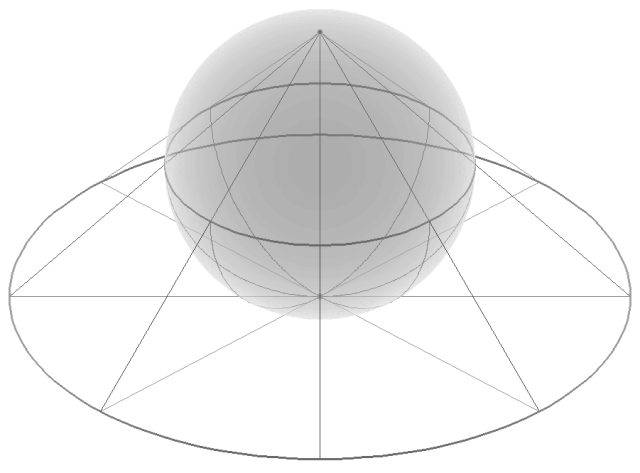
\includegraphics[height = 75mm]{proiezStereo.png}
		\caption{La proiezione stereografica.}
		\label{fig:proiezStereo}
	\end{centering}
\end{figure}

\begin{ese}[Lambert]
	Consideriamo la sezione verticale della sfera.
	Per ogni punto sulla circonferenza in sezione consideriamo una seconda circonferenza che sia centrata nell'origine e che abbia raggio pari alla distanza dell'origine dal punto.
	L'intersezione di tale circonferenza con l'asse \(x\) corrisponde alla proiezione di Lambert.
	\[
		L\colon S^2\setminus\{N\} \to B_2(\bar{0}), \begin{pmatrix}u\\v\end{pmatrix} \mapsto\begin{pmatrix}
			\frac{u\sqrt{4-(u^2+v^2)}}{2} \\[0.3em]
			\frac{v\sqrt{4-(u^2+v^2)}}{2} \\[0.3em]
			\frac{u^2+v^2}{2}-1
		\end{pmatrix}
	\]
	Ora è possibile dimostrare che se \(A\subseteq S^2\) allora l'area di \(A\) corrisponde all'area di \(L(A)\), per cui
	\[
		\dd s = \dd u\,\dd v \iff \norma*{\frac{\pd L^{-1}(u,v)}{\pd u} \wedge \frac{\pd L^{-1}(u,v)}{\pd v}} = 1.
	\]
	Quindi \(\abs{S^2} = \abs{B_2(\bar{0})} = 4\p\).
\end{ese}
%%%%%%%%%%%%%%%%%%%%%%%%%%%%%%%%%%%%%
%TEOREMA DI GULDINO PER LE SUPERFICI%
%%%%%%%%%%%%%%%%%%%%%%%%%%%%%%%%%%%%%
\section{Teorema di Guldino per le superfici}

\begin{teor}{di Guldino per le superfici}{teoremaGuldino}\index{Teorema!di Guldino per le superfici}
	L'area generata dalla rotazione di una curva regolare \(\g\) per un angolo \(\a\) è data dalla lunghezza della curva moltiplicata per la lunghezza dell'area di circonferenza percorsa dal baricentro.
\end{teor}

\begin{proof}
	Dimostriamo il caso in cui la curva è un grafico.
	Avremo quindi \(x=f(z)\) con \(f\in C^1([a,b])\) e la parametrizzazione in coordinate cilindriche
	\[
		\j\colon [a,b] \times [0,\a] \to (0,+\infty) \times S^1 \times \R, \begin{pmatrix}\l\\\q\end{pmatrix} \mapsto 	\begin{pmatrix}
			f(\l) \\
			\q    \\
			\l
		\end{pmatrix}
	\]
	Componiamo con la mappa che ci porta nelle coordinate cartesiane per ottenere
	\[
		\tilde{\j}\colon \begin{pmatrix}\l\\\q\end{pmatrix} \mapsto \begin{pmatrix}
			f(\l)\cos \q \\
			f(\l)\sin \q \\
			\l
		\end{pmatrix}
	\]
	A questo punto basta verificare che l'espressione dell'area corrisponde con la tesi.
	Calcoliamo il prodotto vettore
	\[
		\begin{split}
			\frac{\pd\tilde{\j}}{\pd \l} \wedge \frac{\pd \tilde{\j}}{\pd \q} & = \det  \begin{pmatrix}
				\bar{i}      & \bar{j}      & \bar{k} \\
				f'(\l)\cos\q & f'(\l)\sin\q & 1       \\
				-f(\l)\sin\q & f(\l)\cos\q  & 0
			\end{pmatrix}\\
			& = \bar{i}(-f(\l)\cos\q) - \bar{j}(f(\l)\sin\q) + \bar{k}(f'(\l)f(\l)).
		\end{split}
	\]
	Da cui
	\[
		\norma*{\frac{\pd\tilde{\j}}{\pd \l} \wedge \frac{\pd \tilde{\j}}{\pd \q}} = f(\l)\sqrt{1+\big(f'(\l)\big)^2}.
	\]
	Quindi l'area cercata è
	\[
		\begin{split}
			\int\limits_{\mathclap{[a,b]\times(0,\a)}} f(\l)\sqrt{1+\big(f'(\l)\big)^2}\,\dd \l\,\dd \q & = \int_0^\a \dd \q \int_a^b f(\l)\sqrt{1+\big(f'(\l)\big)^2}\,\dd \l\\
			& = \a\int_a^b f(\l)\sqrt{1+\big(f'(\l)\big)^2}\,\dd \l = \a \int\limits_\g f\,\dd s.
		\end{split}
	\]
	Per trovare l'espressione con il baricentro ci basta moltiplicare e dividere per \(\int\limits_\g \dd s\), ottenendo
	\[
		\a \int\limits_\g \dd s \frac{\int\limits_\g f\,\dd s}{\int\limits_\g \dd s},
	\]
	dove
	\[
		\int\limits_\g \dd s \qquad\text{è per definizione la lunghezza della curva},
	\]
	mentre
	\[
		\frac{\int\limits_\g f\,\dd s}{\int\limits_\g \dd s} \qquad\text{è la distanza del baricentro dall'asse \(z\)},
	\]
	quindi
	\[
		\a \frac{\int\limits_\g f\,\dd s}{\int\limits_\g \dd s} \qquad\text{è la lunghezza dell'area percorsa dal baricentro}.
	\]
\end{proof}

\begin{ese}
	Consideriamo il toro costituito da un tubo di raggio \(r\), il cui centro è distante \(R\) dall'origine.
	Tramite il teorema di Guldino si calcola facilmente che l'area della sua superficie è
	\[
		2\p\,r \cdot 2\p\,R = 4\p^2 r\,R.
	\]
	Dove \(2\p\,r\) è la lunghezza della circonferenza che costituisce la curva regolare che ruota attorno all'asse \(z\).
	Inoltre, dal momento che il baricentro della circonferenza è chiaramente il suo centro, la lunghezza della circonferenza di raggio \(R\) sarà \(2\p\,R\).
\end{ese}
%%%%%%%%%%%%%%%%%%%%%%%%%%%%%%%%%%%%%%%%%%%%%%
%
%LEZIONE 10/05/2016 - UNDICESIMA SETTIMANA (1)
%
%%%%%%%%%%%%%%%%%%%%%%%%%%%%%%%%%%%%%%%%%%%%%%
%%%%%%%%%%%%%%%%%%%%
%TEOREMA DI BROUWER%
%%%%%%%%%%%%%%%%%%%%
\section{Teorema di Brouwer}

\begin{lem}
	Sia \(B=\Set{(x,y) | x^2+y^2 \le 1}\) e supponiamo che \(f\) sia una funzione di classe \(C^2\) su \(\mathring{B}\) e continua su \(B\).
	Se \(f|_{\pd B} = id|_{\pd B}\), allora \(f\) è suriettiva su \(B\).
\end{lem}

\begin{proof}
	Ci basta trovare un assurdo supponendo che \(f\) sia il meno suriettiva possibile, ovvero tale che \(f(B) \subseteq \pd B\).
	Infatti se supponiamo per assurdo che \(f\) sia solo non suriettiva, ovvero che esista \(\bar{x}\in B\) tale che \(\bar{x} \notin f(B)\), possiamo trovare una funzione \(P\) che soddisfi le ipotesi del lemma e che sia del tipo \(P(B) \subseteq \pd B\).

	Infatti \(f(B)\) è compatto in quanto \(B\) è compatto, per cui \(\setc{f(B)}\) è aperto.
	In particolare troviamo \(r>0\) tale che \(B_r(\bar{x})\subseteq \setc{f(B)}\).

	Definiamo la mappa \(P(x)\) in modo che mandi \(x\) nell'intersezione del segmento \(\overline{\bar{x}\,f(x)}\), prolungato dalla parte di \(f(x)\), con la circonferenza \(\pd B\).

	Si mostra facilmente che \(P \in C^2(\mathring{B},\R^2) \cap C(B,\R^2)\), in quanto posso comporre con l'applicazione che proietta \(z\in B\) su \(\pd B\) tramite il segmento che congiunge \(z\) con \(\bar{x}\).
	Tale applicazione è banalmente \(C^2\) in ogni punto diverso da \(\bar{x}\), ma, dal momento che \(\bar{x}\notin f(B)\), avremo \(z=f(x)\neq \bar{x},\,\fa x \in \mathring{B}\).

	Inoltre \(P\) è l'identità sul bordo, in quanto
	\[
		x \in \pd B \implies f(x) = x \implies P(x) = x.
	\]
	Grazie a questo argomento è chiaro che ci basta dimostrare che non esistano mappe \(f\) con la regolarità richiesta e tali che
	\[
		f(x) = x,\,\fa x \in \pd B \qquad\text{e}\qquad f(B) \subseteq \pd B.
	\]
	Scriviamo le generiche componenti della funzione
	\[
		f\colon \begin{pmatrix}x\\y\end{pmatrix} \mapsto 	\begin{pmatrix}
			u(x,y) \\
			v(x,y)
		\end{pmatrix}
	\]
	Per ottenere una contraddizione sfruttiamo il grado di \(f\), definito come
	\[
		\deg f = \int\limits_B \dd u \wedge \dd v.
	\]
	L'idea è calcolare il grado con due procedimenti diversi per ottenere risultati contraddittori.
	Applicando Stokes avremo
	\[
		\begin{split}
			\deg f & = \int\limits_B \dd u \wedge \dd v = \int\limits_B \dd \frac{1}{2}(u\,\dd v -v\,\dd u) = \int\limits_{\pd B} \frac{1}{2}(u\,\dd v - v\,\dd u)\graffito{ricordiamo che su \(\pd B\) si ha \(u(x,y)=x\) e \(v(x,y)=y\).}\\
			& = \int\limits_{\pd B} \frac{1}{2}(x\,\dd y-y\,\dd x) = \p.
		\end{split}
	\]
	D'altronde, sfruttando la definizione di jacobiano,
	\[
		\begin{split}
			\deg f & = \int\limits_B \dd u \wedge \dd v = \int\limits_B (\pd_x u\,\dd x + \pd_y u\,\dd y) \wedge (\pd_x v\,\dd x + \pd_y v\,\dd y)\\
			& = \int\limits_B (\pd_x u\, \pd_y v - \pd_x v\, \pd_y u)\,\dd x \wedge \dd y = \int\limits_B \det  \begin{pmatrix}
				\pd_x u & \pd_y u \\
				\pd_x v & \pd_y v
			\end{pmatrix}\,\dd x\,\dd y
		\end{split}
	\]
	ma
	\[
		\det 	\begin{pmatrix}
			\pd_x u & \pd_y u \\
			\pd_x v & \pd_y v
		\end{pmatrix}\,\dd x\,\dd y
		= 0 \implies \deg f = 0,
	\]
	in quanto le derivate parziali sono parallele.

	Per dimostrare quest'ultima osservazione definiamo
	\[
		g_1(t) = f(x+t,y) \qquad\text{e}\qquad g_2(t) = f(x,y+t),
	\]
	tali funzioni costituiscono una curva in quanto \(f(B)\subseteq \pd B\).
	In particolare \(g_1'(0)\) e \(g_2'(0)\) sono entrambi vettori tangenti a \(f(x,y)\) e sono pertanto paralleli.
	D'altronde, per la regola della catena,
	\[
		g_1'(0) = f'(x+t,y)|_{t=0} \begin{pmatrix}1\\0\end{pmatrix} = \begin{pmatrix}\pd_x u\\\pd_x v\end{pmatrix}
		\qquad\text{e}\qquad
		g_2'(0) = f'(x,y+t)|_{t=0} \begin{pmatrix}0\\1\end{pmatrix} = \begin{pmatrix}\pd_y u\\\pd_y v\end{pmatrix}.
	\]
	Quindi ho trovato che \(\deg f = \p = 0\) che è assurdo.
\end{proof}

\begin{teor}{di Brouwer}{teoremaBrouwer}\index{Teorema!di Brouwer}
	Sia \(B=\Set{(x,y) \in \R^2 | x^2+y^2 \le 1}\) e supponiamo che \(f\) sia una funzione di classe \(C^2\) su \(\mathring{B}\) e continua su \(B\).
	Se \(f(B)\subseteq B\) allora esiste \(x\in B\) tale che \(f(x)=x\).
\end{teor}

\begin{proof}
	Supponiamo per assurdo che \(f(x)\neq x,\,\fa x\in B\).
	Definiamo la mappa \(P(x)\) in modo che mandi \(x\) nell'intersezione del segmento \(\overline{x\,f(x)}\), prolungato dalla parte di \(x\), con la circonferenza \(\pd B\).
	Come nel caso del lemma precedente si mostra facilmente che \(P\in C^2(\mathring{B},\R^2)\cap C(B,\R^2)\).
	Inoltre vale \(P(x)=x\) se \(x\in \pd B\).
	Per cui le ipotesi del lemma sono soddisfatte e \(P\) dovrebbe risultare suriettiva.
	Ma ciò è ovviamente assurdo in quanto \(P(B)=\pd B\).
\end{proof}

\begin{oss}
	Il caso monodimensionale con \(f\colon [0,1] \to [0,1]\) continua segue dal teorema del valore intermedio applicato a \(g(x)=x-f(x)\).

	Infatti \(g(0)=-f(0)\le0\) in quanto \(f(0)\in[0,1]\).
	D'altronde \(g(1)=1-f(1)\ge 0\) in quanto \(f(1)\in[0,1]\).
	Quindi per il teorema del valore intermedio esiste \(x\in[0,1]\) tale che \(g(x)=0\), ovvero \(f(x)=x\).
\end{oss}
%%%%%%%%%%%%%%%%%%%%%%%%%%%%%%%%%%%%%%%%%%%%
%TEOREMA DELLA DIVERGENZA IN TRE DIMENSIONI%
%%%%%%%%%%%%%%%%%%%%%%%%%%%%%%%%%%%%%%%%%%%%
\section{Teorema della divergenza in tre dimensioni}

\begin{teor}{della divergenza in tre dimensioni}{divergenza3D}\index{Teorema!della divergenza in tre dimensioni}
	Sia \(T\) un unione finita di domini aperti e normali rispetto a tutti e tre gli assi.
	Sia \(F\) un'applicazione di classe \(C^1\) su \(T\) e continua sulla chiusura \(\overline{T}\).
	Allora
	\[
		\iiint\limits_T \divg F\,\dd x\,\dd y\,\dd z = \iint\limits_{\pd T} \Braket{F,n}\,\dd S.
	\]
\end{teor}

\begin{proof}
	Scriviamo \(T\) come dominio normale rispetto a \(z\),
	\[
		T = \Set{(x,y,z) | (x,y) \in D, \a(x,y) < z < \b(x,y)}.
	\]
	Utilizzando le formule di riduzione, avremo
	\[
		\begin{split}
			\iiint\limits_T \pd_z F_3 (x,y,z)\,\dd x\,\dd y\,\dd z & = \iint\limits_D \dd x\,\dd y \int_{\a(x,y)}^{\b(x,y)}\pd_z F_3 (x,y,z)\,\dd z\graffito{tramite il TFC}\\
			& = \iint\limits_D \Big[F_3\big(x,y,\b(x,y)\big)-F_3\big(x,y,\a(x,y)\big)\Big]\,\dd x\,\dd y.
		\end{split}
	\]
	Ora vorremmo calcolare \(\iint\limits_{\pd T}F_3 n_3\,\dd S\) e verificare che coincide con il risultato appena trovato.
	Osserviamo che in quanto dominio normale rispetto alle \(z\), possiamo suddividere \(\pd T\) in tre superfici \(S_1,S_2\) e \(S_3\), dove
	\begin{itemize}
		\item \(S_1\) è la calotta superiore parametrizzata da \(\y\colon D \to \R^3, (u,v)\mapsto \big(u,v,\b(u,v)\big)\);
		\item \(S_2\) è la calotta inferiore parametrizzata da \(\y\colon D \to \R^3, (u,v)\mapsto \big(u,v,\a(u,v)\big)\);
		\item \(S_3\) è la superficie che congiunge \(S_1\) e \(S_2\).
	\end{itemize}
	In particolare avremo
	\[
		\iint\limits_{\pd T}F_3 n_3\,\dd S = \iint\limits_{S_1} F_3 n_3\,\dd S + \iint\limits_{S_2} F_3 n_3\,\dd S + \iint\limits_{S_3} F_3 n_3\,\dd S.
	\]
	Ora
	\[
		\iint\limits_{S_3} F_3 n_3\,\dd S = 0,
	\]
	in quanto \(n_3 = 0\) su \(S_3\).
	Per verificarlo, parametrizziamo \(S_3\) e calcoliamo il vettore normale.
	Siano \(\g\colon S^1 \to \pd D, t\mapsto \big(\g_1(t),\g_2(t)\big)\) e
	\[
		\y\colon \Set{(t,s) | t \in S^1, \a\big(\g(t)\big) < s < \b\big(\g(t)\big)}, (t,s) \mapsto \big(\g_1(t),\g_2(t),s\big).
	\]
	A questo punto basta calcolare il prodotto vettore e verificare che è nullo nella componente verticale.

	Per \(S_1\) abbiamo già trovato una parametrizzazione, calcoliamo il prodotto vettore
	\[
		\frac{\pd \y}{\pd u} \wedge \frac{\pd \y}{\pd v} = \det \begin{pmatrix}
			\bar{i} & \bar{j} & \bar{k}  \\
			1       & 0       & \pd_u \b \\
			0       & 1       & \pd_v \b
		\end{pmatrix}
		= -\bar{i} \pd_u \b - \bar{j} \pd_v \b + \bar{k}
	\]
	Dal momento che la terza componente è \(1\) avremo che, per normalizzazione
	\[
		n_3 = \frac{1}{\norma{\pd_u \y \wedge \pd_v \y}},
	\]
	da cui
	\[
		\begin{split}
			\iint\limits_{S_1} F_3 n_3\,\dd S & = \iint\limits_D F_3\big(u,v,\b(u,v)\big) \frac{1}{\norma{\pd_u \y \wedge \pd_v \y}} \norma{\pd_u \y \wedge \pd_v \y}\,\dd u\,\dd v\\
			& = \iint\limits_D F_3 \big(u,v,\b(u,v)\big)\,\dd u\,\dd v.
		\end{split}
	\]
	Resta da calcolare su \(S_2\), ma ovviamente osserveremo un comportamento del tutto analogo; eccetto il segno del versore che sarà negativo così da farlo puntare all'esterno.
	Quindi infine
	\[
		\iint\limits_{\pd T} F_3 n_3\,\dd S = \iint\limits_D F_3\big(u,v,\b(u,v)\big)\,\dd u\,\dd v - \iint\limits_D F_3\big(u,v,\a(u,v)\big)\,\dd u\,\dd v,
	\]
	che coincide proprio con quanto calcolato inizialmente.

	Con lo stesso procedimento si verifica che
	\[
		\iiint\limits_T \pd_y F_2(x,y,z)\,\dd x\,\dd y\,\dd z = \iint\limits_{\pd T} F_2 n_2\,\dd S \qquad\text{e}\qquad \iiint\limits_T \pd_x F_1(x,y,z)\,\dd x\,\dd y\,\dd z = \iint\limits_{\pd T} F_1 n_1\,\dd S,
	\]
	dal momento che il dominio è per ipotesi normale rispetto a tutti gli assi.
	Da cui la tesi.
\end{proof}

\begin{oss}
	In \(\R^{2n}\) posso sempre trovare un campo non nullo con divergenza nulla.
	Ad esempio in \(\R^2\) posso considerare
	\[
		F(x,y) = 	\begin{pmatrix}
			0  & 1 \\
			-1 & 0
		\end{pmatrix} \begin{pmatrix}x\\y\end{pmatrix}
		\implies \divg F \begin{pmatrix}x\\y\end{pmatrix} = \divg \begin{pmatrix}y\\-x\end{pmatrix} = \pd_x(y) + \pd_y (x) = 0.
	\]
	In generale possiamo sempre considerare la matrice
	\[
		J = \begin{pmatrix}
			0  & 1                            &    &   &                              &        \\
			-1 & 0                            &    &   & \makebox(0,0){\text{\Huge0}} &        \\
			   &                              & 0  & 1 &                              &        \\
			   &                              & -1 & 0 &                              &        \\
			   & \makebox(0,0){\text{\Huge0}} &    &   & \ddots                       &        \\
			   &                              &    &   &                              & \ddots
		\end{pmatrix}
	\]
\end{oss}

\begin{ese}
	Troviamo la relazione tra l'area e il volume della sfera.
	Consideriamo
	\[
		F(x,y,z) = \begin{pmatrix}x\\y\\z\end{pmatrix}.
	\]
	Applicando il teorema della divergenza avremo
	\[
		\iiint\limits_{B_1^2(\bar{0})}\divg F\,\dd x\,\dd y\,\dd z = \iint\limits_{S^2} \Braket{F,n}\,\dd S.
	\]
	Dove
	\[
		\divg F = 3 \implies \iiint\limits_{B_1^2(\bar{0})}\divg F\,\dd x\,\dd y\,\dd z = 3 \abs*{B_1^2(\bar{0})}.
	\]
	D'altronde il versore normale alla sfera è \((x,y,z)\), in quanto posso definire \(S^2\) come la superficie associata a \(G\colon x^2+y^2+z^2=1\), da cui
	\[
		n = \frac{\nabla G}{\norma{\nabla G}} = \frac{2(x,y,z)}{2\sqrt{x^2+y^2+z^2}} = (x,y,z),
	\]
	in quanto \((x,y,z)\in S^2 \implies x^2+y^2+z^2 = 1\).
	Quindi
	\[
		\Braket{F,n} = x^2+y^2+z^2 = 1 \implies \iint\limits_{S^2} \dd S = \text{ area}(S^2).
	\]
	Ovvero area\((S^2) = 3\abs*{B_1^2(\bar{0})}\), infatti \(4\p = \frac{4}{3}\p\).
\end{ese}

\begin{ese}
	Calcoliamo il flusso di \(F\) attraverso \(\pd T\), con
	\[
		F(x,y,z) = \begin{pmatrix}0\\y\,z\\x\end{pmatrix} \qquad\text{e}\qquad T=\Set{(x,y,z) | x^2+y^2\le z^2, z\ge 0, x^2+y^2+z^2 \le 2y}.
	\]
	Per il teorema della divergenza
	\[
		\iint\limits_{\pd T} \Braket{F,n}\,\dd S = \iiint\limits_T \divg F\,\dd x\,\dd y\,\dd z = \iiint\limits_T z\,\dd x\,\dd y\,\dd z.
	\]
	Ora \(T=\Set{(x,y,z) | (x,y)\in B_1\big((0,1)\big), \sqrt{x^2+y^2} \le z \le \sqrt{1-x^2-(y-1)^2}}\).
	Inoltre vale la condizione implicita
	\[
		\sqrt{x^2+y^2} \le \sqrt{1-x^2-(y-1)^2} \iff x^2+y^2 \le y,
	\]
	ovvero
	\[
		T=\Set{(x,y,z) | (x,y)\in B_{\frac{1}{2}}\big((0,1/2))\big), \sqrt{x^2+y^2} \le z \le \sqrt{1-x^2-(y-1)^2}}.
	\]
	Da cui
	\[
		\iiint\limits_T z\,\dd x\,\dd y\,\dd z = \iint\limits_{\mathclap{B_{1/2}\big((0,1/2)\big)}}\dd x\,\dd y \int_{\sqrt{x^2+y^2}}^{\sqrt{2y-(x^2+y^2)}}z\,\dd z = \iint\limits_{\mathclap{B_{\frac{1}{2}}\big((0,1/2)\big)}} y-(x^2+y^2)\,\dd x\,\dd y.
	\]
	A questo punto basta passare in coordinate polari per ottenere il risultato di \(\p/32\).
\end{ese}
%%%%%%%%%%%%%%%%%%%%%%%%%%%%%%%%%%%%%%%%%%%%%%
%
%LEZIONE 11/05/2016 - UNDICESIMA SETTIMANA (2)
%
%%%%%%%%%%%%%%%%%%%%%%%%%%%%%%%%%%%%%%%%%%%%%%
\begin{prop}{Relazione tra volume e area del bordo}{relazioneVolumeArea}
	Sia \(D\) un dominio regolare tale che \(D\subseteq B_R(\bar{0})\).
	Allora
	\[
		\abs{D} \le \frac{R}{3} \text{ area}(\pd D).
	\]
\end{prop}

\begin{proof}
	Consideriamo il campo identità
	\[
		F\colon \R^3 \to \R^3, F(x,y,z) = \begin{pmatrix}x\\y\\z\end{pmatrix}.
	\]
	Applicando il teorema della divergenza,
	\[
		\iiint\limits_D \divg F\,\dd x\,\dd y\,\dd z = \iint\limits_{\pd D} \Braket{F,n}\,\dd S,
	\]
	dove
	\[
		\iiint\limits_D \divg F\,\dd x\,\dd y\,\dd z = 3\abs{D},
	\]
	mentre, tramite la disuguaglianza di Cauchy-Schwarz,
	\[
		\iint\limits_{\pd D} \Braket{F,n}\,\dd S \le \iint\limits_{\pd D} \underbrace{\norma{F}}_{\le R} \underbrace{\norma{n}}_{= 1}\,\dd S \le R \iint\limits_{\pd D}\dd S = R \text{ area}(\pd D).\qedhere
	\]
\end{proof}

\begin{oss}
	Se \(D\) è la sfera vale l'uguaglianza.
\end{oss}
%%%%%%%%%%%
%APPENDICE%
%%%%%%%%%%%
\section{Appendice}

\begin{defn}{Laplaciano}{laplaciano}\index{Laplaciano}
	Sia \(f\) una funzione di classe \(C^2\).
	Il \emph{laplaciano}, o operatore di Laplace, associato ad \(f\), si definisce come la divergenza del gradiente di \(f\).
\end{defn}

\begin{notz}
	Si scrive
	\[
		\Delta f = \divg \nabla f.
	\]
\end{notz}

\begin{prop}{Prima equazione di Green}{primaEqGreen}\index{Prima equazione di Green}
	Sia \(D\) un dominio regolare in \(\R^3\).
	Siano \(R\colon D \to \R^3\) e \(\y\colon D \to \R\) una funzione di classe \(C^1\) su \(D\) e continua fino al bordo.
	Supponiamo che
	\[
		R(x,y,z) = (\pd_x \j,\pd_y \j, \pd_z \j),
	\]
	con \(\j\) una funzione di classe \(C^2\) su \(D\) e \(C^1\) fino al bordo.
	Allora
	\[
		\iiint\limits_D \big(\Braket{\nabla \y,\nabla \j} + \y\Delta \j\big)\,\dd x\,\dd y\,\dd z = \iint\limits_{\pd D} \y\,\pd_n \j\,\dd S.
	\]
\end{prop}

\begin{proof}
	Calcoliamo la divergenza di \(\y\,R\):
	\[
		\begin{split}
			\divg (\y\,R) & = \divg(\y\,\pd _x\j, \y\,\pd_y \j,\y\,\pd_z \j)\\
			& = (\pd_x \y\,\pd_x \j + \pd_y \y\,\pd_y \j + \pd_z \y\,\pd _z \j) + \y(\pd_{x\,x}^2 \j + \pd_{y\,y}^2 \j + \pd_{z\,z}^2 \j)\\
			& = \Braket{\nabla \y,\nabla \j} + \y \,\Delta \j.
		\end{split}
	\]
	Ovvero \(\divg(\y\,\Delta \j) = \Braket{\nabla \y,\nabla \j} + \y\,\Delta \j\).
	Applicando il teorema della divergenza a \(F= \y\,\Delta \j\) otteniamo
	\[
		\iiint\limits_D \divg F\,\dd x\,\dd y\,\dd z = \iint\limits_{\pd D} \Braket{F,n}\,\dd S,
	\]
	dove \(\Braket{F,n} = \y \Braket{\nabla \j,n} = \y\,\pd_n \j\).
	Ovvero
	\[
		\iiint\limits_D \big(\Braket{\nabla \y,\nabla \j} + \y\Delta \j\big)\,\dd x\,\dd y\,\dd z = \iint\limits_{\pd D} \y\,\pd_n \j\,\dd S.\qedhere
	\]
\end{proof}

\begin{prop}{Seconda equazione di Green}{secondaEqGreen}\index{Seconda equazione di Green}
	Sia \(D\) un dominio regolare in \(\R^3\).
	Siano \(\j,\y\colon D \to \R\) due funzioni di classe \(C^2\) su \(D\) e \(C^1\) fino al bordo.
	Allora
	\[
		\iiint\limits_D (\y\,\Delta \j - \j\,\Delta \y)\,\dd x\,\dd y\,\dd z = \iint\limits_D (\y\,\pd_n \j - \j\,\pd_n \y)\,\dd S.
	\]
\end{prop}

\begin{proof}
	Dal momento che \(\j\) e \(\y\) soddisfano vicendevolmente le ipotesi della prima equazione di Green, avremo
	\[
		\iiint\limits_D \big(\Braket{\nabla \y,\nabla \j} + \y\Delta \j\big)\,\dd x\,\dd y\,\dd z = \iint\limits_{\pd D} \y\,\pd_n \j\,\dd S,
	\]
	e
	\[
		\iiint\limits_D \big(\Braket{\nabla \j,\nabla \y} + \j\Delta \y\big)\,\dd x\,\dd y\,\dd z = \iint\limits_{\pd D} \j\,\pd_n \y\,\dd S.
	\]
	Per ottenere la tesi è sufficiente sottrarre membro a membro.
\end{proof}

\begin{defn}{Funzione armonica}{funzioneArmonica}\index{Funzione!armonica}
	Una funzione \(f\colon D \to \R\) di classe \(C^2\) si dice \emph{armonica} se il suo laplaciano è costantemente nullo.
	Ovvero
	\[
		\Delta f = 0,\,\fa x \in D.
	\]
\end{defn}

\begin{teor}{Funzione armonica nulla sul bordo}{funzioneArmonicaNullaBordo}
	Sia \(h\colon D \to \R\) una funzione armonica. Supponiamo che \(h\) sia costantemente nulla su \(\pd D\).
	Allora \(h\equiv 0\) su \(D\).
\end{teor}

\begin{proof}
	In quanto armonica \(h\) è certamente una funzione di classe \(C^2\).
	Ricordando che \(\Delta h = 0\) e che \(h|_{\pd D} \equiv 0\), applichiamo la prima equazione di Green con \(\j = \y = h\):
	\[
		\iiint\limits_D \abs{\nabla h}^2\,\dd x\,\dd y\,\dd z = 0,
	\]
	per cui \(\nabla h \equiv 0\), ovvero, per Lagrange, \(h\equiv\) cost.
	Ma \(h\equiv 0\) su \(\pd D\), per cui \(h \equiv 0\) su \(D\).
\end{proof}

\begin{teor}{Funzioni armoniche coincidenti sul bordo}{funzioniArmonicheCoincidentiBordo}
	Siano \(h_1,h_2\colon D \to \R\) due funzioni armoniche.
	Supponiamo che \(h_1 \equiv h_2\) su \(\pd D\).
	Allora \(h_1 \equiv h_2\) su \(D\).
\end{teor}

\begin{proof}
	Basta applicare il teorema precedente alla funzione armonica \(h_1-h_2\).
\end{proof}

\begin{teor}{Ulteriori proprietà delle funzioni armoniche}{ulterioriPropArmoniche}
	Sia \(h\colon D \to \R\) una funzione armonica.
	Supponiamo che \(\pd_n h \equiv 0\) su \(\pd D\).
	Allora \(h \equiv \) cost su \(D\).
\end{teor}

\begin{proof}
	Applichiamo la prima formula di Green con \(\y=\j=h\)
	\[
		\iiint\limits_D \abs{\nabla h}^2\,\dd x\,\dd y\,\dd z = 0,
	\]
	da cui \(\abs{\nabla h} = 0\), ovvero, per Lagrange, \(h\equiv \) cost.
\end{proof}

\begin{cor}
	Se \(h_1,h_2\) sono funzioni armoniche su \(D\), tali che \(\pd_n h_1 \equiv \pd_n h_2\) su \(\pd D\);
	allora \(h_1-h_2 \equiv \) cost.
\end{cor}

\begin{proof}
	Basta applicare il teorema precedente alla funzione armonica \(h_1-h_2\).
\end{proof}

\begin{ese}[Gabbia di Faraday]
	Se consideriamo una struttura tale che \(W\) sia il campo elettrico interno e \(V\) quello esterno.
	Supponendo che \(\Delta W = 0\) nella struttura e \(W\equiv \) cost sul bordo, allora \(W\equiv \) cost.
	Per cui il campo \(\nabla W\) è nullo.
\end{ese}